
%%% Local Variables: 
%%% mode: latex
%%% TeX-master: "paper"
%%% End: 


We define a set of \emph{local} formulae. A formula is local if its groundings relate any number of observed ground atoms to exactly one hidden ground atom. For example, a grounding of the local formula 
\[lemma(p,+l_1) \wedge lemma(a,+l_2) \Rightarrow hasRole(p,a)\]
can be seen in the Markov Network of Figure \ref{fig:local2}. It connects a hidden \emph{hasRole} ground atom to two observed \emph{lemma} ground atoms. Note that the ``+'' prefix for variables indicates that the different weight for each possible pair of lemmas $(l_1,l_2)$.

% This formula is used during the argument classification stage which in our model is related to the hidden predicate $hasRole$. Given a sentence, this formula will create a ground formulua for each combination of lemmas and positions where the formula is true. This can be seen in the Figure \ref{fig:local2}\footnote{Segment of sentence from training corpora.} where there are two instances of the predicate. You can notice that the only hidden predicate involved on each of this formulae is the $hasLabel$ predicate.
% \begin{figure}
% \caption{MLN for lemmas of predicate and argument}
% \label{fig:local1}
% \end{figure}
% Remember that the MLN relates the FOL forumula with a weighted feature. For this formulae the weighted feature consists of both lemmas. 

\begin{figure}
\begin{center}
    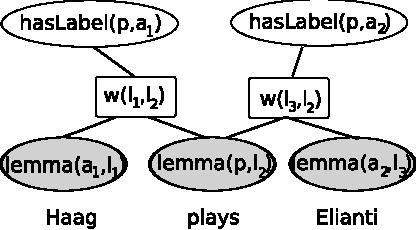
\includegraphics[scale=.70]{LocalFormula2}
\end{center}
\caption{Factor graph for example of local formula.}
\label{fig:local2}
\end{figure}

For the \emph{hasRole} and \emph{role} predicates we defined local formulae which aimed to reproduce the standard features used in previous work~\citep{xue04calibrating}. This also required us to develop dependency-based versions of the constituent-based features such as the syntactic path between predicate and argument, as proposed by \cite{xue04calibrating}. 

The remaining hidden predicates, \emph{isPredicate}, \emph{isArgument} and \emph{sense}, have local formulae that relate their ground atoms to properties of a contextual window around the token the atom corresponds to. For this we used the information provided in the open track training corpus of the shared task (i.e. both versions of lemma and POS tags plus a coarse version of the POS tags). 

Instead of describing the local feature set in more detail we refer the reader to our MLN model files.\footnote{\url{http://thebeast.googlecode.com/svn/mlns/conll08}} They can be both used as a reference and as input to our Markov Logic Engine\footnote{\url{http://thebeast.googlecode.com}}, and thus allow the reader to easily reproduce our results. We believe that this is another advantage of explicitly separating model and algorithms by using first order probabilistic logic languages.

% Additionaly, we created formulae using the information provided in the open track training corpora. In particular, we define formulae to capture the relations provided by the dependency parsing. For this, we extracted the subcategorization of each word and the minimum path between words. There were versions with dependency labels and without them. This was done for each of the hidden predicates with exception of $frameLabel$. The $WordNet$ labels provided in the open track were also used to define local formulae, in particular for the $hasLabel$ and $role$ predicates.

% We also implemented the a prune heuristic of ~\cite{xue04calibrating} and create a observable predicate which signals if a word shouln't be consider as an argument . This predicate was use to define local formulae for the $hasLabel$ and $role$ hidden predicates. Finally, we create a hidden predicate to identify when the word was unknown (i.e., a word occurs less than two times in the train corpus). We define some formulae with this predicate for the $role$ predicate. (Maybe point out to the pml files).





 



